\section{Friction}

Friction is a force that resists the movement of two contacting surfaces sliding relative to each other. Frictional forces act tangential to the surface at the point of contact and act in opposition to the possible or existing motion between the surfaces. 

\blue{Insert content from the TAM 212 page Friction and Damping - Introductory equation box}

\subsection{\red{Static Friction}}

Examples of coefficients of static friction: 

\begin{figure*}[!h]
\centering
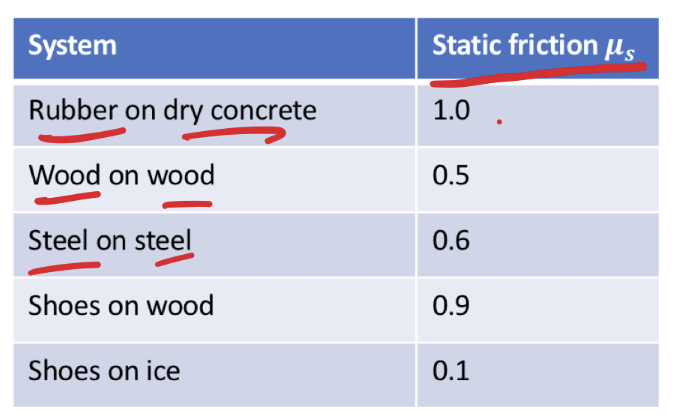
\includegraphics[angle=0, width=3 in]{FrictionFigures/ExampleCoeff.png}
\vspace{-2mm}
\caption{\small \blue{Taken from TAM 210 Lecture 26}}
\vspace{-3mm}
\label{Fig:ExampleCoeff}
\end{figure*}

\blue{This might be a good place to add practical examples - maybe how engine brakes use friction? And another thing about how cartilage in your joints has very little friction (like ice on ice!) which allows for joint movement.}

In TAM 210/211, we will focus on dry friction. Dry friction occurs between two surfaces with \textbf{no} lubricating fluid between them. 

Static friction is the friction between two bodies when there is no movement between them. 

\subsection{Tipping vs. Slipping}

\begin{figure*}[!h]
\centering
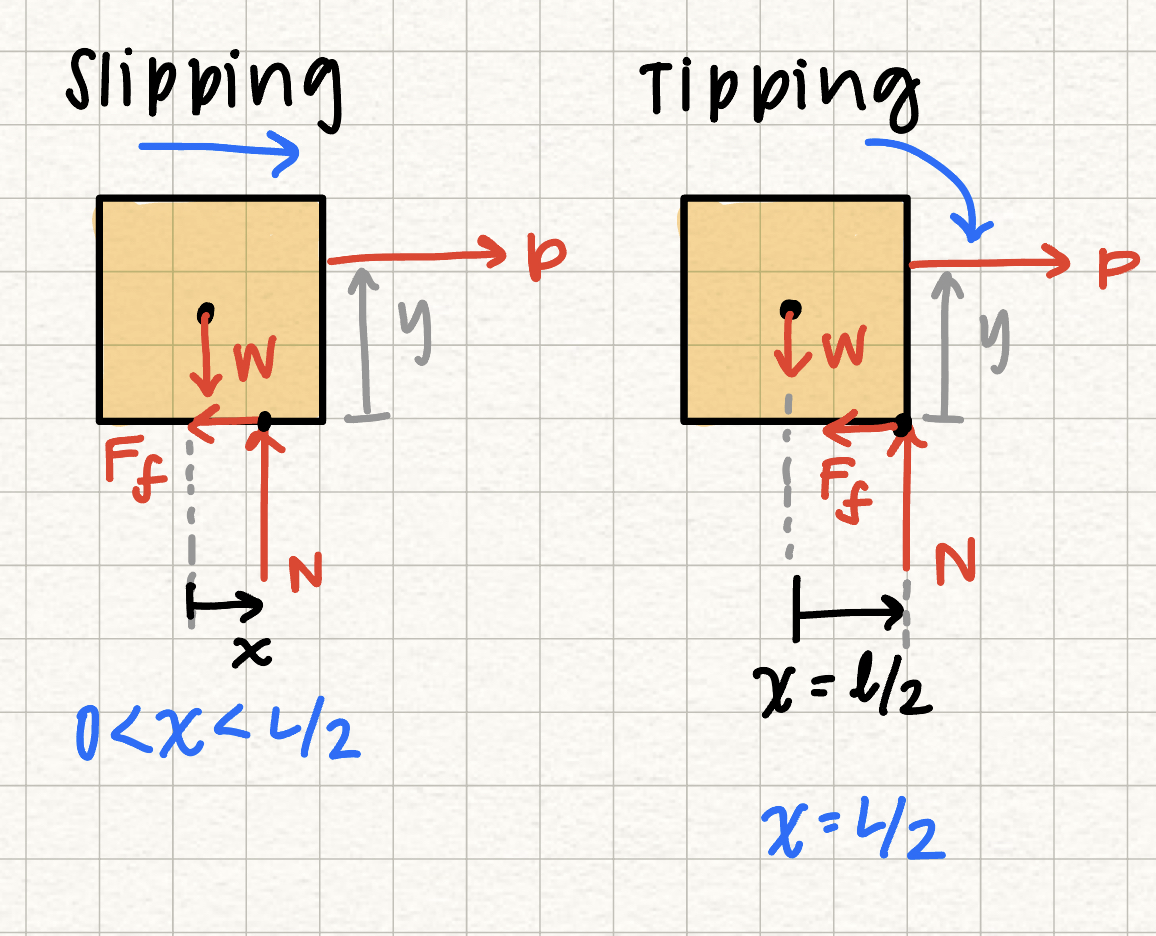
\includegraphics[angle=0, width=\textwidth]{FrictionFigures/TipSlip.png}
\vspace{-2mm}
\caption{\small \blue{Taken from TAM 210 Lecture 27}}
\vspace{-3mm}
\label{Fig:TipSlip}
\end{figure*}

%From Lecture 27

